% Portable Software -> new repository
\section{Software Implementation}
\label{sec: implementation}

% Custom command for inline code
\newcommand{\code}[1]{\texttt{#1}}

Given that the machine learning part of the software is modulized as "Climate Reconstruction AI" (CRAI), the neural net's setup, training and evaluation are outsourced.
Thus, the process for a single specific dataset of one station could be written pretty straightforwardly with a \code{NetCDF} file of the station data at hand if there is sufficient access to ERA5 data.
A Jupyter notebook would be sufficient as a way to start.
However, dealing with different stations leads to different preprocessed files for numerous evaluation and training processes, and the situation becomes increasingly intricate.
Management is needed to allow for pipelines to be run in a structured way, ensuring that the input settings for CRAI are set dynamically and that all the necessary files are created and stored in the right place.
Thus, it appears natural to implement a set of functions and structure the process through an object-oriented approach.
As seen in \autoref{fig: training_pipeline} and \autoref{fig: infilling_pipeline}, pipelines for training and infilling have many similarities, and a lot of the implemented methods can be reused.
Moreover, the model's evaluation is conducted similarly for infilling and validation.
The only distinction between these two pipelines is in the final step of displaying the results."

This chapter is about laying the foundation through the implementation of the different steps of the pipeline as classes and functions. Thereupon, in chapter \autoref{sec: process_orchestration}, the next abstraction level of the software into classes that handle the execution of the different steps is described.

The following subsections highlight the critical steps of the pipeline and how their functionality evolves.
It does not cover the detailed embedding of the methods in their classes, nor is it explicitly mentioned where temporary folders would be created to establish a philosophy where each step of the pipeline is implemented independently and can be connected in a higher-level class.
The methods are not necessarily intended to be used in any arbitrary order but rather in accordance with the desired pipelines.
However, the modularity allows for a better understanding and cleaner code, which is essential when developing another layer of abstraction later.

\begin{figure}
    \centering
    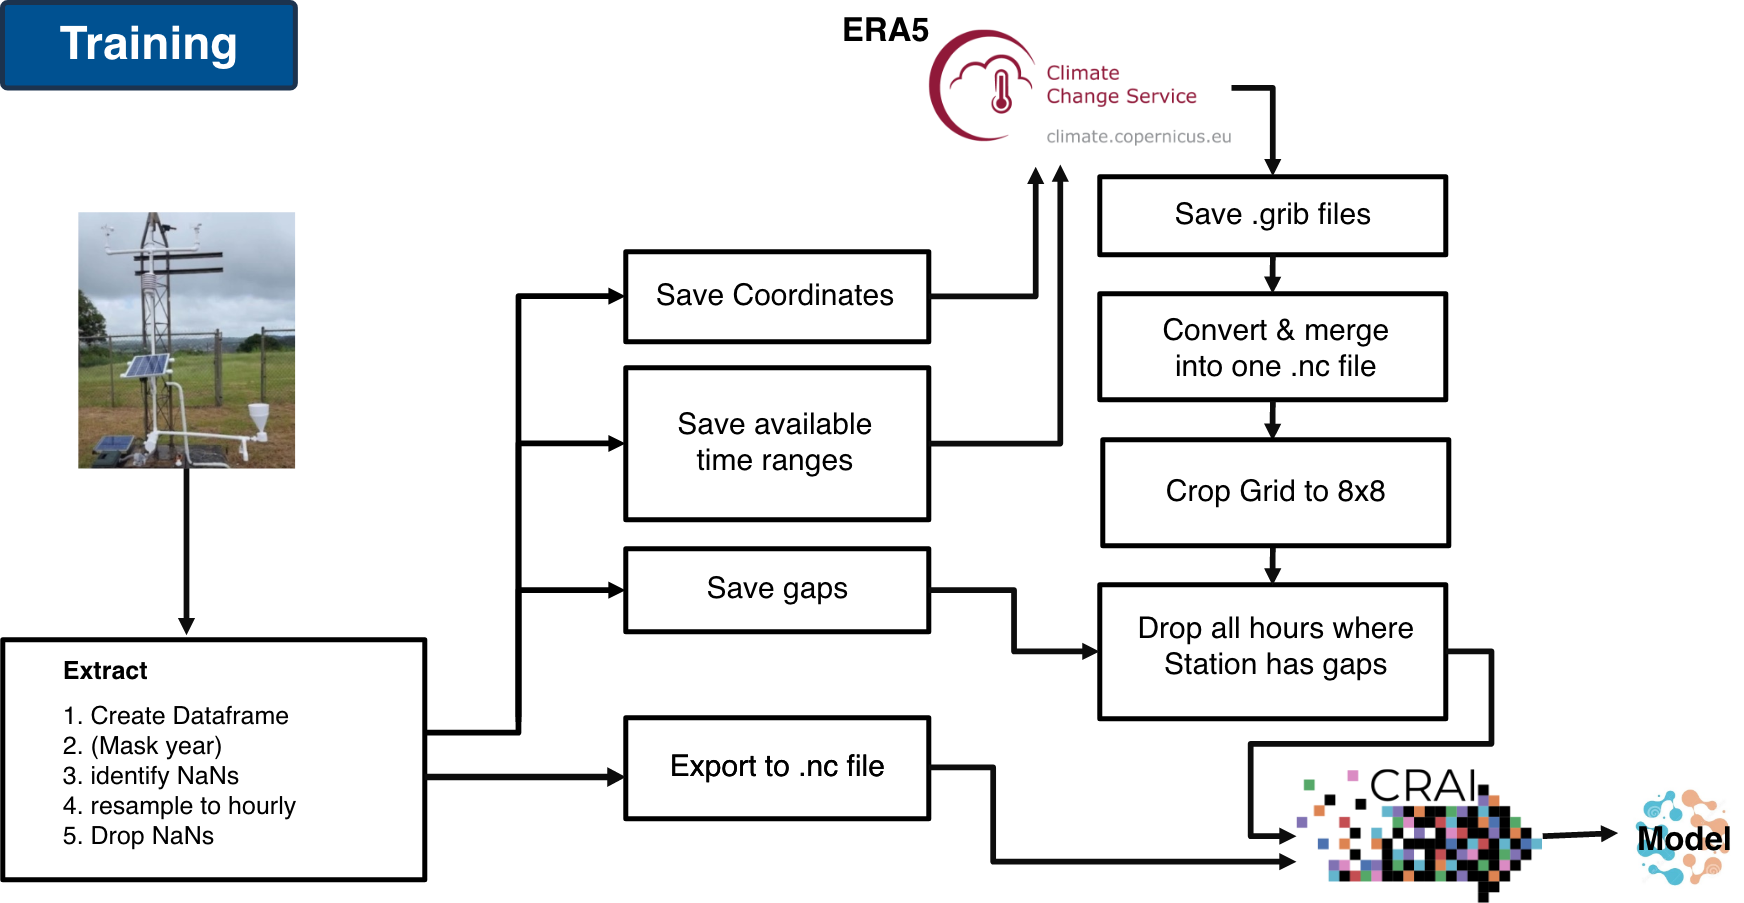
\includegraphics[width=450pt]{resources/images/training_pipeline.png}
    \caption{Pipeline to train a model.}
    \label{fig: training_pipeline}
\end{figure}

\begin{figure}
    \centering
    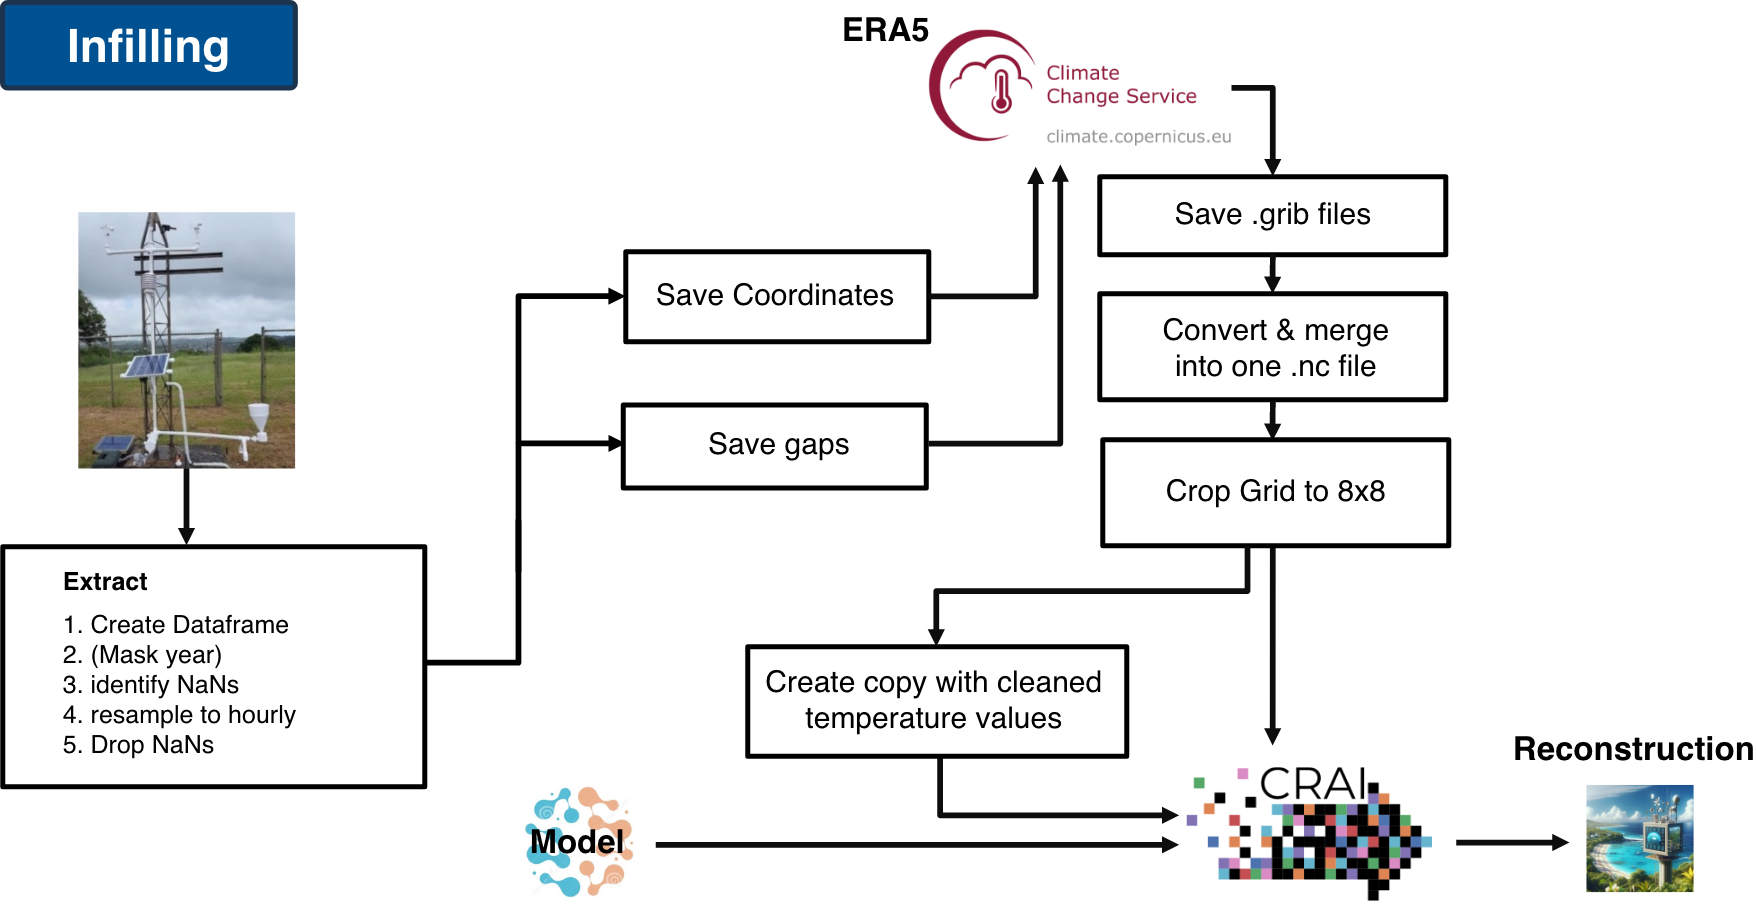
\includegraphics[width=450pt]{resources/images/infilling_pipeline.png}
    \caption{Pipeline to reconstruct weather data using a model.}
    \label{fig: infilling_pipeline}
\end{figure}

\subsection{Station Data Submission and Conversion}

The station data for the 3D-printed weather stations provided by NCAR comes in delimited text files, with one file per day and a text-based metadata file holding information such as the station name, latitude, longitude, and elevation. 
The data files (.dat files) contain one column per sensor and one row per minute.

A class \code{DatToNcConverter} is implemented with the following functionalities:
First, it takes the \code{.dat} files and the metadata file into a directory and parses them. 
Second, the data is processed, including dropping missing values, resampling to an hourly frequency, and converting from Celsius to Kelvin to match ERA5. 
This is easiest in a pandas dataframe. 
Third, it converts the data to a \code{NetCDF} file, which is the format used by the ERA5 data and the CRAI module. 
The \code{NetCDF} file is structured in a way that stores the data in a 3D array with the dimensions time, latitude, and longitude. 
The metadata is stored as global attributes in the \code{NetCDF} file. 
Fourth, it converts some dataframes back to \code{.dat} files after the reconstruction of measurements to match the original format when infilling.

The resampling to hourly frequency is the most complex use case, as it includes many design decisions.
Missing values are marked with \code{-999.99}, so in the first step, these values are marked as \code{NaN}.
However, the data quality is not controlled by default, and there could be values that should be marked as missing but are not.
Thus, the NCAR consulted to mark \code{0.00} °C as \code{NaN}.
For stations like Barbados, this wouldn't be a realistic value, but even for regions where 0°C degrees are reached often, it is unlikely to measure exactly \code{0.00}, meaning the amount of correct data lost through marking \code{0.00} as \code{NaN} is limited.
Additionally, by agreement with the NCAR, everything above or under \code{± 45°C} is marked as \code{NaN}.
To compensate for peaks in the data, aggregating the minutes using a median instead of a mean is a good idea; \code{numpy.median()} would return \code{NaN} if any value is \code{NaN}, while \code{numpy.nanmedian()} would ignore \code{NaN}s.
It is best to have a custom aggregate function using \code{numpy.nanmedian()}.

For the use case of converting the data back to a \code{.dat} file, the dataframe is stored directly in the converter object as the original dataframe. Only the detection of \code{NaN}s and the aggregation to hourly values are done before, as the use case lies in the infilling task, and the reconstruction gives hourly values.
After saving the original state, any transformation of units (Celsius to Kelvin), renaming of columns and most importantly, the actual clearing of the \code{NaN}s take place.
Fundamentally, in between the first and last measurements, rows exist for all minutes, even if measurements are missing.
However, if the station had severe issues, it is possible that between the first and last record, there are even rows or files missing.
To assure that the original dataframe, where the NaNs are not supposed to be cleared, will have rows for all hours, a handy method provided by the Python pandas module is used:

\begin{lstlisting}
    self.original_df = self.original_df.reindex(
        pd.date_range(start = self.dataframe.index.min(), end = self.dataframe.index.max(), freq = "h"))
\end{lstlisting}

A class \code{Station} is implemented to hold the metadata and the pandas dataframe of the station data.
It includes the converter itself, which it can then use automatically.
The class primarily manages access to the different files and the data, both before and after the conversion.
Additionally, it detects gaps in the data, providing a simple list of hours where data is missing for infilling purposes.
For training use cases, it also lists the months where at least some data is available, which is convenient when using the API to obtain ERA5 data for the station.

\begin{lstlisting}[caption=Gap Detection in Station Class, label=lst: find_gaps]
def find_gaps(self) -> None:
available_hour_steps = self.df.index
all_hour_steps = self.converter.original_df.index
# find all hours between the first and last hour that are missing
missing_hours = all_hour_steps.difference(available_hour_steps)
return missing_hours.tolist()
\end{lstlisting}

\begin{lstlisting}[caption=Detection of available ranges in Station Class, label=lst: available_ranges]
def get_all_months_in_df(self) -> None:
# return all (year, month) tuples in the dataframe
periods = self.df.index.to_period('M').unique().tolist()
month_dict = {}
for period in periods:
    if period.year not in month_dict:
        month_dict[period.year] = []
    month_dict[period.year].append(period.month)
return month_dict
\end{lstlisting}

\subsection{Copernicus Climate Data Store - CDS API}
\label{sec: cds_api}

The Copernicus Climate Data Store (CDS) is a service by the European Centre for Medium-Range Weather Forecasts (ECMWF).
The CDS API provides open source access to the ERA5 data, allowing users to download the data for a specific location and time period.
After creating an account online an API Key can be obtained for free and with the python module 'cdsapi' data can then be downloaded easily in \code{.grib} format. 

\begin{lstlisting}[caption=Download Hook for ERA5 Data, label=lst: download_hook]
import cdsapi

class Era5DownloadHook:
    
    def __init__(self, lat, lon):
        self.cds = cdsapi.Client(
            url="https://cds.climate.copernicus.eu/api/v2",
            key=f"{os.getenv('UID')}:{os.getenv('API_KEY')}"
        )
        self.lon, self.lat = lon, lat

    def _download(cds, date_info, save_to_file_path):
        cds.retrieve(
            'reanalysis-era5-single-levels',
            {
                "product_type": "reanalysis",
                "format": "grib",
                "variable": "2m_temperature",
                "area": [
                    self.lat + 1, # limit north
                    self.lon - 1 % 360, # limit west
                    self.lat - 1, # limit south
                    self.lon + 1 % 360, # limit east
                ],
                "year": date_info.get("years"),
                "month": [f"{month:02d}" for month in date_info.get("months")],
                "day": [f"{day:02d}" for day in date_info.get("days")],
                "time": [f"{hour:02d}:00" for hour in date_info.get("hours")]

            }, save_to_file_path)



\end{lstlisting}

As can be seen in the \autoref{lst: download_hook}, the request encompasses, in addition to dynamic spatial cropping and temporal selection, the fundamental details of our requirement: to download 2-meter temperature data in \code{.grib} format from the ERA5 reanalysis.
In the class \code{Era5DownloadHook}, further the following is implemented to download a few hours in a day at once.

\begin{lstlisting}[caption=Download Hours in Same Day in Download Hook Class, label=lst: download_hours_in_same_day]
    def download_hours_in_same_day(self, year, month, day, hours, target_folder):
        self._download({
            "years": [year],
            "months": [month],
            "days": [day],
            "hours": hours
        }, f"{year}_{month}_{day}.grib")
\end{lstlisting}

When using a variation of \autoref{lst: download_hours_in_same_day}to download a month or an entire year, it becomes obvious why the \autoref{lst: available_ranges} is so helpful.

In the \autoref{lst: download_hook}, it can be seen that the regional selection is always +/- 1 degree around the Station location.
Because of the grid interval of 0.25°, this ensures that the downloaded area always includes at least 9x9 grid points, such that when cropping to an 8x8 selection the station can always be centered, even without exact knowledge of the coordinates of the desired grid points prior to requesting. 


\subsection{Data Preprocessing}

As pointed out in \autoref{sec: cds_api}, the data is downloaded in \code{.grib} format.
Using the program \code{cdo}, the data can be quickly converted to \code{.nc} format with the following simple command:

\begin{lstlisting}
cdo -f nc copy {source_path} {nc_path}
\end{lstlisting}

However, to have the "temperature at surface" variable name unified as \code{"tas"} in the \code{NetCDF} file, the following command can be used:

\begin{lstlisting}[caption=Renaming Variable in \code{NetCDF} File, label=lst: rename_variable]
    import xarray as xr
    import subprocess

    def _rename_variable(self, var_name, tas_name, input, output):
        rename_variable_command = \
            f"cdo chname,{var_name},{tas_name} {input_path} {output_path}"
        subprocess.run(rename_variable_command, shell=True)
        
    ds = xr.open_dataset(input_path)
    if 'var167' in ds.variables:
        _rename_variable('var167', 'tas', input_path, output_path)
    elif '2t' in ds.variables:
        _rename_variable('2t', 'tas', input_path, output_path)

\end{lstlisting}

Then the files are merged using 

\begin{lstlisting}
    cdo cat {temp_dir_path}/*.nc {era5_target_file_path}
\end{lstlisting}

before the data is cropped to the 8x8 grid around the station location, as described in \Ref{subsec: data_preprocessing}.

For training the data, it needs to be assured that the ERA5 data does not include timesteps that the nc file of the station data does not include so that the time dimensions are identical.
This is done in two steps:
First, the ERA5 data is cropped using a start-to-end date approach using the first and last date of the station data.
Then, all hours that were missing in the station dataset, identified by the find gaps method in \autoref{lst: find_gaps}, are removed from the ERA5 data.
This is done using the python module \code{xarray} and deleting the timesteps in batches of up to 1000 timesteps, as deleting all at once could cause issues.

The station data should have the same dimensions as the ERA5 data, so a method is applied that copies the ERA5 dataset and replaces all the temperature values with the measured value from the corresponding hour in the station data.

For evaluating the model, the same preparation of ERA5 data is done in a validation procedure.
However, instead of passing the station data as expected output to the model, the file will not be filled with the measured values but with \code{NaN}s.

When evaluating the model not for validation but to infill missing values, the ERA5 data of course, needs to be prepared differently of course.
Instead of requesting monthly data from the \code{cdsapi}, it is requesting only the missing hours day by day, such that the time-dimension is directly as desired, and preprocessing only needs to handle the conversion and geographical cropping.

\subsection{Handling the Model Output}
Because CRAI is using the encode, decode architecture as described in \autoref{subsec: cnn}, the output file in \code{NetCDF} format that the model produces includes not only one temperature value per timestep but has the same dimensions as the input ERA5 file meaning it uses the same 8x8 grid with 64 temperature values.
However, since it was trained on input files where the ground truth was also laid on the 8x8 grid, the 64 temperature values in the output data of the model tend to be highly similar.
To make this transformation but primarily for practical reasons, the output file will be converted to a pandas dataframe again, where the calculated mean of the 64 values is stored.
Two different methods were implemented, creating different dataframes, as the model was evaluated in two different use cases.
One is the validation of the model, where the output is compared to the ground truth, and as in \autoref{sec: results} to ERA5 nearest grid point.
The other is the infilling of missing values, where the output is not compared but the original dataframe of the station data is updated with reconstructed values.
Both methods take the output file of the model as input, while the validation method also needs to take the groud truth and ERA5 into account.
For the ground truth, the file created by the \code{DatToNcConverter} is used, while for the ERA5 data the file that has been passed to the model is used.
The ground truth file still uses the coordinates of the station and is not stretched to the 8x8 grid, as was done during the training.
Therefore the method to create the validation dataframe \code{era5\_vs\_reconstructed\_comparision\_to\_df} can obtain the station coordinates from that file and then decide which grid point in the ERA5 data is the nearest to the station.
To highlight one last core method, \code{plot\_n\_steps\_of\_df} is very useful during validation and powered the standardized plotting of the results (\autoref{subsec: validation_results}).
It takes in the dataframe returned by \code{era5\_vs\_reconstructed\_comparision\_to\_df}, and plots the temperature values of the station, the ERA5 nearest grid point, and the reconstructed values for a specific number of timesteps.
One handy feature is that if a number of timesteps is given, it will plot only that amount of timesteps, allowing for a more detailed view of the results.
It chooses the extract of \code{n} consecutive timesteps randomly, leading to the weekly extract plots in \autoref{subsec: validation_results}.
In all the created plots in \autoref{subsec: validation_results}, the RMSE and the correlation coefficient are calculated and displayed in the title of the plot,
that has also been done in the method \code{plot\_n\_steps\_of\_df}.
Lastly, the method is also able to plot the temperature differentials instead of the absolute values when told to do so by an optional boolean flag.
Then, of course after the calculation of the RMSE and correlation coefficient, it offsets the values
In all these functionalities, the plotting method heavily benefits from the creation of the dataframe, as it can slice along the time dimension conveniently.